\documentclass[tikz]{standalone}

\usetikzlibrary{shapes.arrows}

\begin{document}
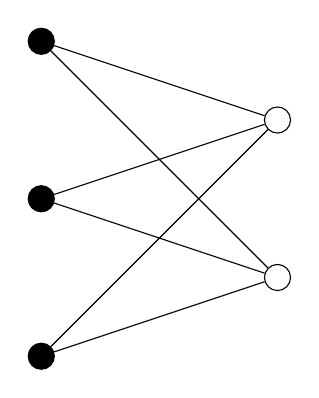
\begin{tikzpicture}[every node/.style={circle, draw}]
    \node[fill=black] (x1) at (0, 0) {};
    \node[fill=black] (x2) at (0, 2) {};
    \node[fill=black] (x3) at (0, 4) {};
    
    \node (y1) at (3, 1) {};
    \node (y2) at (3, 3) {};

    \foreach \i in {1, 2, 3}
        \foreach \j in {1, 2}
            \draw (x\i) -- (y\j);
\end{tikzpicture}

\end{document}